\documentclass[11pt, A4paper, english]{article}
\usepackage[utf8]{inputenc}
\usepackage[T1]{fontenc}
\usepackage{babel}
\usepackage{amsmath}
\usepackage{amsfonts}
\usepackage{amsthm}
\usepackage[colorlinks]{hyperref}
\usepackage{listings}
\usepackage[pdftex]{color}
\usepackage{hyperref}
\usepackage{graphicx}
\usepackage{cite}
\usepackage{float}
\usepackage{multicol}
\usepackage{subcaption}
\usepackage[margin=2cm]{geometry}

\definecolor{dkgreen}{rgb}{0,0.6,0}
\definecolor{gray}{rgb}{0.5,0.5,0.5}
\definecolor{daynineyellow}{rgb}{1.0,0.655,0.102}
\definecolor{url}{rgb}{0.1,0.1,0.4}

\lstset{
frame=tb,
language=Python,
aboveskip=3mm,
belowskip=3mm,
showstringspaces=false,
columns=flexible,
basicstyle={\small\ttfamily},
numbers=none,
numberstyle=\tiny\color{gray},
keywordstyle=\color{blue},
commentstyle=\color{daynineyellow},
stringstyle=\color{dkgreen},
breaklines=true,
breakatwhitespace=true,
tabsize=3
}

%The exemples under is for paths in windows and the second is in linux
\lstset{inputpath = /home/torstein/Dokumenter/UiO/Fys-Stk4155/"Project 1"/Class}

\graphicspath{{/home/torstein/Dokumenter/UiO/Fys-Stk4155/"Project 1"/Run/}}
\hypersetup{colorlinks, urlcolor=url}

%This is how to put in codefiles
%\lstinputlisting{<Filnavn type kodefil>}
%To crope lines shown insert
%firstline = <linenumber>, lastline = <linenumber>
%as kwarg

%This is how to put in pictures
%\includegraphics[width=12.6cm,height=8cm]{<Filnavn type png>}
%To crop a picture insert 
%trim={<left> <lower> <right> <upper>}, clip
%as kwargs

\author{
Torstein Solheim Ølberg \\
Institute for Theoretical Astrophysics, University of Oslo \\
P.O. Box 1029 Blindern 0315 Oslo, Norway
%F.eks:
%Institute for Theoretical Astrophysics, University of Oslo \\
%P.O. Box 1029 Blindern 0315 Oslo, Norway
}
\title{On Linear Regression Methods for a Terrain Dataset}

\begin{document}
	
\maketitle
\tableofcontents
\clearpage
	
	\section{Abstract}
%Here the article is briefly summarized, mentioning some background, the methods and data used as well as notable results - keep it short and to the point.
Performing analysis in machine learning is a powerful tool in many different fields of science. For this it is important to familiarise oneself with different methods of analysis for different problems. In this project I look at three methods for approximating a 3D data set, Ordinary Least Squares, Ridge and Lasso regression. Use Mean Square Error, Bootstrap resampling and Cross Validation resampling to estimate which models fit a made up dataset, and a terrain dataset the best, and find that it is the $20$th degree OLS fit which best mimic the datasets. As for Ridge and Lasso we find a $\lambda = -0.5$ and $p = $, and $\lambda = 0.1$ respectively, but the Lasso model doesn't converge for any polynomial degree and is thus useless.
	
	
	\begin{multicols}{2}
		\section{Introduction}
%Why are we doing this exercise, what are our assumptions, what do we want to accomplish?
The field of data analysis has been revolutionised by the introduction of machine learning in the middle of the 20th century. This process revolves around the approximation of models to some set of data by the brute force use of computers. In this report we will try study three simple linear regression models, the Ordinary Least Squares (OLS), Ridge and Lasso regression methods, on a made up data set and then use it on a real dataset and try to find the best possible method. The article itself will start with a description of the made up data produced from the Franke function and the real data from the USA Geological survey. Then the scaling, model building and different analysis methods will be described. Finally the results are presented and discussed and the total contents of the article will be summarised.
		
		\section{Data Description}
The first dataset we make ourselves, produced by the so called Franke function. This is a function consisting of the sum of four exponentials and produces a plane dataset since it takes two separate variables $x$ and $y$.
		\begin{align}
f(x, y) =& \frac{3}{4} e^{\left( - \frac{\left( 9x - 2 \right)^2}{4} - \frac{\left( 9y - 2 \right)^2}{4} \right)} \\
\nonumber +& \frac{3}{4} e^{\left( - \frac{\left( 9x + 1 \right)^2}{49} - \frac{\left( 9y + 1 \right)^2}{10} \right)} \\
\nonumber +& \frac{1}{2} e^{\left( - \frac{\left( 9x - 7 \right)^2}{4} - \frac{\left( 9y - 3 \right)^2}{4} \right)} \\
\nonumber -& \frac{1}{5} e^{\left( - \left( 9x - 4 \right)^2 - \left( 9y + 7 \right)^2 \right)}
		\end{align}
We choose to make the dataset with $x$ and $y$ values from $[0, 1]$, and choose linearly $10^4$ pairs of points. We should also make the dataset more realistic by adding some noise to the data. For this we choose to draw a set of random numbers, equal to the number of data points, drawn from a normal distribution with mean value $0$ and standard deviance equal to $1$. Then we add these points to our Franke function values. \\
The second, and "real" dataset is taken from the United States Geological Survey \cite{USGS}. Here we find an elevation dataset from the SRTM 1 Arc-second global group from the region around the Oslo Fjord.  It is simply a measurement of the height in meters above sea level. We extract the small part in the top of the left corner showing Finnemarka. You can see the dataset in figure \ref{Finnemarka}
		\begin{figure}[H]
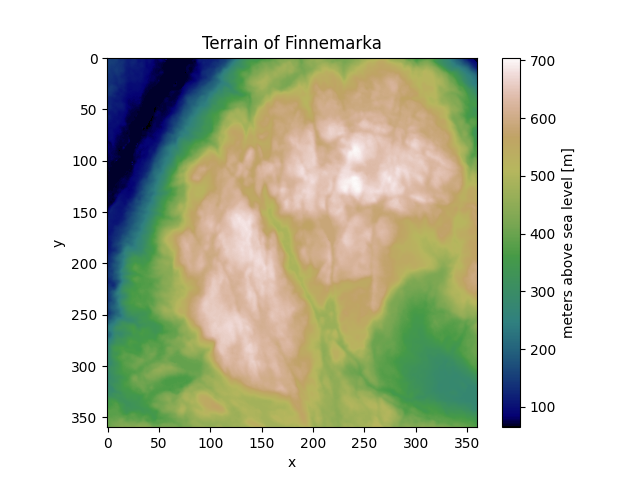
\includegraphics[width=\linewidth, height=7cm]{Figure20.png}
\caption{The Finnemarka elevation dataset}
\label{Finnemarka}
		\end{figure}

		\section{Methods}
%How did you obtain the data, what methods did you use? Describe your work process. If you performed an experiment using specific equipment, describe your setup.
			\subsection{Scaling}
It is useful to scale our data before we perform any approximation of our dataset, as this will help us to account for problems with outliers and particularly large values when we fit, which otherwise could make the data very dependant upon these points. We will use the simple standard scaling from \textit{Sklearn.preprocessing} called scale. This subtracts the mean value of the data from the data points.

			\subsection{Building the Model}
When performing a linear regression, we want a model on the form
			\begin{equation}
z = \sum_{i = 0}^{p} \sum_{j = 0}^{i} \beta_{\sum_{k = 0}^{i} + j} x^{i - j}y^{j}
			\end{equation}
This might look odd, but is just a compact way of writing a standard 2 dimensional $p$ degree polynomial. for $p = 2$ this is simply
			\begin{equation*}
z = \beta_0 + \beta_1 x + \beta_2 y + \beta_3 x^2 + \beta_4 xy + \beta_5 y^2 
			\end{equation*}
To perform this regression we need to set up a vector $\vec{X}$ on the form
			\begin{equation}
\vec{X} = \left[ \begin{matrix}
\sum_{i = 0}^{p} \sum_{j = 0}^{i} x_0^{i - j}y_0^{j} \\
\sum_{i = 0}^{p} \sum_{j = 0}^{i} x_1^{i - j}y_1^{j} \\
\dots \\
\sum_{i = 0}^{p} \sum_{j = 0}^{i} x_n^{i - j}y_n^{j} \\
\end{matrix} \right]
			\end{equation}
where $n$ are the number of $x, y$ pairs in the dataset. \\
Then we can split our dataset into two groups, a training and a test group. We use $20\%$ of our dataset as a test and the rest as training group.

				\subsubsection{Ordinary Least Squares}
Now we are prepared to model our data with the OLS method. This is a simple task where we approximate the $\beta$ values by finding the minimum value of the cost function
				\begin{equation*}
C(\vec{\beta}) =  \frac{1}{n} \left\{ \left( \vec{y} - \vec{X} \vec{\beta} \right)^{T} \left( \vec{y} - \vec{X} \vec{\beta} \right) \right\}
				\end{equation*}
It is simple to show, by taking the derivative of $C$ that the minimum point can be found from
				\begin{equation}
\vec{\beta} = \left( \vec{X}^T \vec{X} \right)^{-1} \vec{X}^T \vec{y}
				\end{equation}
as long as $\vec{X} \vec{X}^T$ is invertible. If they are not, we can approximate them by the Moore-Penrose pseudo-inverse instead, and use this result. To compute the inverse we use the \textit{numpy.linalg} function pinv \cite{Pinv}.

			\subsubsection{Ridge Regression}
Another way to perform the Linear regression is the Ridge method. This is almost the same as the OLS, except the introduction of a constant $\lambda$ times the norm of $\beta$ into the cost function.
				\begin{equation*}
C(\vec{\beta}) =  \frac{1}{n} \left\{ \left( \vec{y} - \vec{X} \vec{\beta} \right)^{T} \left( \vec{y} - \vec{X} \vec{\beta} \right) \right\} + \lambda ||\beta||_2^2
				\end{equation*}
This gives us a way to find beta in the same way as for the OLS except with a $\lambda$ times an identity matrix
				\begin{equation}
\vec{\beta} = \left( \vec{X}^T \vec{X} + \lambda \vec{I} \right)^{-1} \vec{X}^T \vec{y}
				\end{equation}
With the same assumption as for the OLS.

			\subsubsection{Lasso Regression}
The last regression method is the Lasso regression, where we define the cost function to be equal to
				\begin{equation*}
C(\vec{\beta}) =  \frac{1}{n} \left\{ \left( \vec{y} - \vec{X} \vec{\beta} \right)^{T} \left( \vec{y} - \vec{X} \vec{\beta} \right) \right\} + \lambda ||\beta||_1
				\end{equation*}
where we have used $||\beta||_1 = \sum_{i} |\beta|$. This doesn't have a numerical solution to the derivative of $C$ like the other two methods. However, the python package \textit{sklearn} has a useful method \textit{linear\_model.Lasso} \cite{Lasso} which we can use to perform this minimalisation task for us. \\

			\subsection{Analysis methods}
We need to find a way to measure which method is the best at approximating our dataset, and to do this a simple measure might be to look at the Mean Square Error and use this as our prediction error.
				\subsubsection{Mean Square Error}
The MSE is simply the mean value of the square of the errors between the approximations and the measured values.
				\begin{equation}
MSE = \frac{1}{n} \sum_{i} \left( z_i - \hat{z}_i \right)^2
				\end{equation}
where $z$ are the measured values and $\hat{z}$ are the true values. \\
				\subsubsection{R Squared}
We can also calculate the $R^2$ value of the model, which is defined as
				\begin{equation}
R^2 = 1 - \frac{\sum_{i} \left( z_i - \hat{z}_i \right)^2}{\sum_{i} \left( z_i - \bar{\hat{z}} \right)^2}
				\end{equation}
$\bar{\hat{z}}$ is the mean value of the approximations. \\
				\subsubsection{Bootstrap Resampling}
A more complicated, but still quite simple way to find the best fit model is to perform the bootstrap resampling method. This method is based on the assumption that we can perform the prediction of our data a number of times $a$, where we each time choose a random subset of the test and training group, with resampling of the training data. Thus we get $a$ new train and test groups, with the same size as the original once, and we can find the MSE for each and averaging over all the MSEs. From this we can also split the MSE into three other parts, the Bias, the Variance and the variance of the error. To get this, we can look at the MSE
				\begin{align*}
MSE =& \frac{1}{n} \sum_{i} \left( z_i - \hat{z}_i \right)^2 \\
=& \text{E}\left[ \left( \vec{z} - \hat{\vec{z}} \right)^2 \right]
				\end{align*}
where E denotes the expected value. If we add $E[\hat{\vec{z}}] - E[\hat{\vec{z}}]$ inside the square and perform the squaring, we can rewrite this as 
				\begin{align*}
MSE =& \text{E}\left[ \left( \hat{\vec{z}} - E[\hat{\vec{z}}] \right)^2 \right. \\
&+ \left( \vec{z} - E[\hat{\vec{z}}] \right)^2 \\
&\left.+ 2 \left( E[\hat{\vec{z}}] - \vec{z} \right) \left( \hat{\vec{z}} - E[\hat{\vec{z}}] \right) \right]
				\end{align*}
The estimated value of an estimated value is simply the estimated value, and the estimated value of a measured value is simply the measured value. This lets us rewrite the above as
				\begin{align*}
MSE =& \text{E}\left[ \left( \hat{\vec{z}} - E[\hat{\vec{z}}] \right)^2 \right] \\
&+ E \left[ \left( \vec{z} - E[\hat{\vec{z}}] \right)^2 \right] \\
&+ 2 \left( E[\hat{\vec{z}}] - \vec{z} \right) \left( E[\hat{\vec{z}}] - E[\hat{\vec{z}}] \right) \\
=& \text{E}\left[ \left( \hat{\vec{z}} - E[\hat{\vec{z}}] \right)^2 \right] \\
&+ E \left[ \left( \vec{z} - E[\hat{\vec{z}}] \right)^2 \right] \\
=& \text{Var}(\hat{\vec{z}}) + \sigma^2 + \text{Bias}(\vec{z}, \hat{\vec{z}})^2
				\end{align*}
The Last step her is just splitting the left term into the variance of the model and the variance of the assumed noise. This result gives us the bias and the variance
				\begin{align}
\text{Bias} =& \frac{1}{n} \sum_i \left( z_i - E[\hat{\vec{z}}] \right)^2 \\
\text{Var} =& \frac{1}{n} \sum_i \left( \hat{\vec{z}} - E[\hat{\vec{z}}] \right)^2
				\end{align}
As we can see, the bias is simply the average of the difference between the measured value and the estimated approximation value. The Variance is the same, but the measured value is exchanged for the approximated value. \\
We can then calculate the MSE, bias and variance and plot them as a function of our polynomial degree, to find at what value the bias and variance has the optimal values. \\

				\subsubsection{Cross Validation}
Last of all, we can perform the so called Cross Validation resampling method (CV). Here we shuffle and perform a random split of data into test and training groups a number of times $N$ and calculate the MSE every time. Then we find the mean of this value, by summing all the results and dividing by $N$, and use this as our MSE estimate.	

				\subsection{Performing the analysis}
First we will perform the analysis methods for OLS, finding the best fit polynomial degree, which would be the polynomial degree giving the lowest error values. Then we will find the optimal lambda for Ridge and Lasso, using a degree of 5. This we do for the Franke function to test our method, afterwords we can perform the same thing for the terrain data. Last, we use this lambdas for the terrain data to find the optimal degree and compare the best fit models for OLS, Ridge and Lasso. Optimally we would have liked to perform the Lasso and Ridge regression for an interval of degree and $\lambda$ at the same time, to be sure the combination we get is the best possible. This would however take much more time to run than we have time for so we will simply perform one at a time and assume this is close to the right result.

		\section{Results}
			\subsection{Franke function}
%What were your clear-cut results? - Present them in a clear and concise manner, waiting with the discussion of them for later. Here you present calculations, figures and tables of data, output of code, etc.
Performing the OLS estimate of the Franke dataset with a first through fifth degree polynomial, we get $R^2$ values as shown in figure \ref{R2}. In this plot we see that the function increases in the beginning and then reaches a top, falls drastically and then rises a little again. This also gives us the visualisation of the approximation seen in figure \ref{3D_Franke} where the left plot is of the actual Franke function with noise added, and the right is the OLS approximation to the function for the fifth degree. We see that there are a lot of difference between the function with noise and the model.
			\begin{figure}[H]
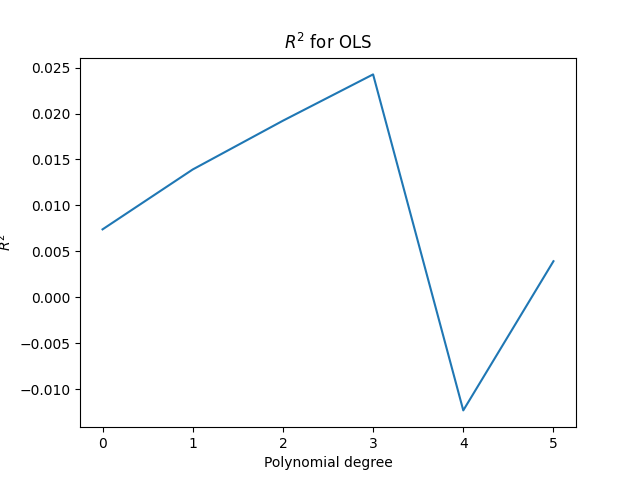
\includegraphics[width=\linewidth, height=7cm]{Figure00.png}
\caption{$R^2$ as a function of the polynomial degree for the OLS method applied on the Franke function. We see that the function rises until 3rd degree, then falls to a negative value for 4th degree and rises for the 5th one again.}
\label{R2}
			\end{figure}
			\begin{figure}[H]
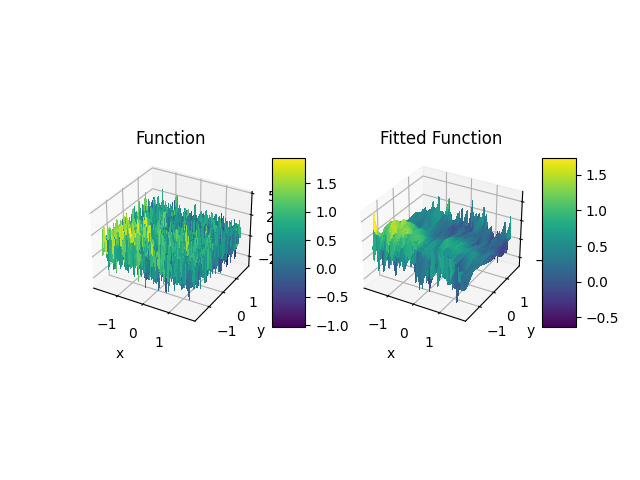
\includegraphics[width=\linewidth, height=7cm]{Figure10.png}
\caption{To the left is the Franke function with noise and to the right is the fitted approximation with OLS method for a fifth degree polynomial. They vary a lot from each other.}
\label{3D_Franke}
			\end{figure}
When we perform the OLS for a range of polynomial degrees between zero and 30, we get a MSE as a function for the polynomial degree for both the training and test data. This plot is seen in figure \ref{MSE_OSL}.
			\begin{figure}[H]
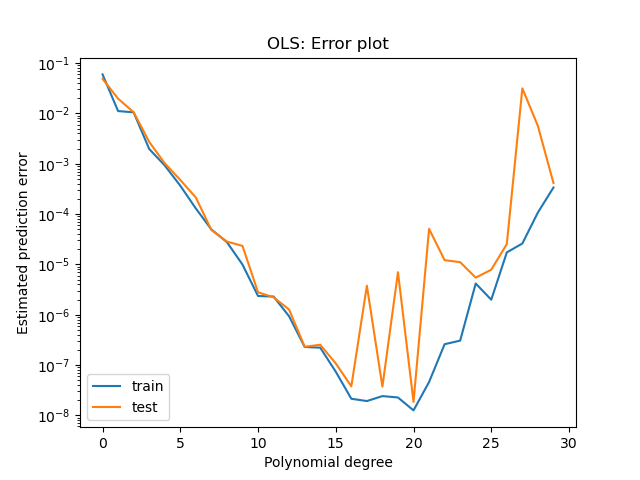
\includegraphics[width=\linewidth, height=7cm]{Figure01.png}
\caption{MSE as a function of polynomial degree for both the test and train dataset groups. Train data has its error reduced with higher degree, but the test data rises after 8th degree.}
\label{MSE_OSL}
			\end{figure}
We see that the training data error is reduced the higher value of the polynomial we get, until around 20th degree where it stabilises. However the test data has a stable curve until around 8th degree where it starts to vary drastically. This gives us a lowest error value at 7th degree for both sets. \\
The Bootstrap analysis for the OLS gives us a plot of the MSE, Bias and Variance, which we can see in figure \ref{Bootstrap_OLS}.
			\begin{figure}[H]
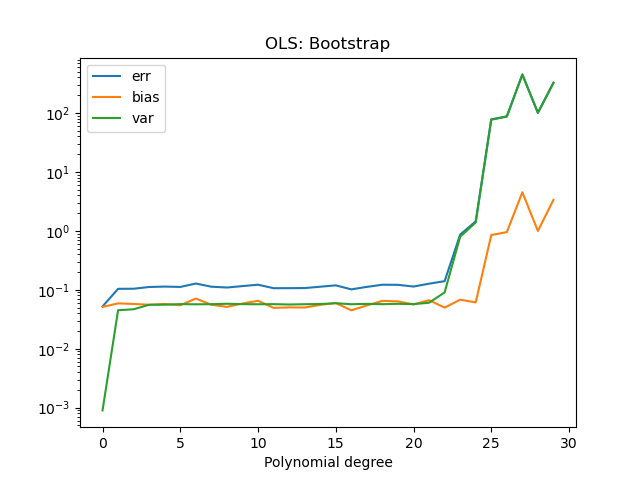
\includegraphics[width=\linewidth, height=7cm]{Figure02.png}
\caption{Bootstrap MSE, bias and variance for OLS. Error is stable until around 7th degree and then blows up, bias is stable until 14th degree and then blows up and variance increases slowly until 14th degree when it overlaps with error and blows up.}
\label{Bootstrap_OLS}
			\end{figure}
Here we see a similar evolution to the test curve in the MSE plot. The error and bias stay almost constant until about 8th level, where it stats to increase and vary drastically. The exception is the variance which increases slowly the whole time but blows up after 10th degree. \\
The Cross Validation gives us a MSE which we can compare with the MSE of Bootstrap. We plot these two in figure \ref{CV_OLS}.
			\begin{figure}[H]
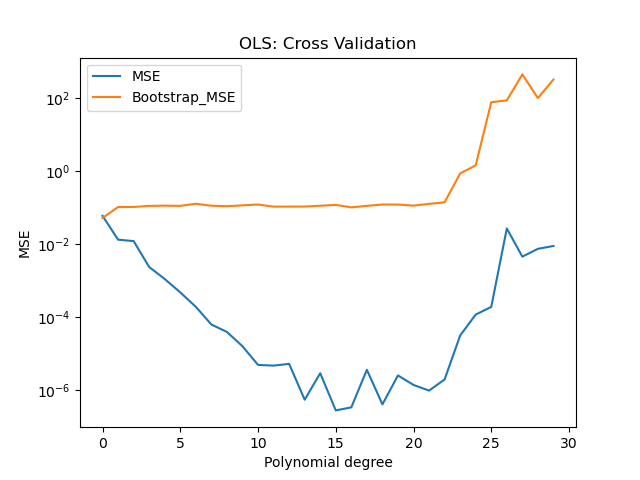
\includegraphics[width=\linewidth, height=7cm]{Figure03.png}
\caption{Cross Validation MSE estimate for OLS compared with the Bootstrap MSE. Both are very similar and almost constant until around 7th degree where the bootstrap start to blow up. Then later at 10th degree the CV also start to increase. The bootstrap error increases much faster than the CV MSE.}
\label{CV_OLS}
			\end{figure}
We see that the CV is stable like the bootstrap was, but start to increase later than the bootstrap, waiting until around 1st degree before it increases more slowly but blows up eventually. \\
For the Ridge we get a MSE as a function for the $\lambda$ for both the training and test data which we can see in figure \ref{MSE_Ridge}.
			\begin{figure}[H]
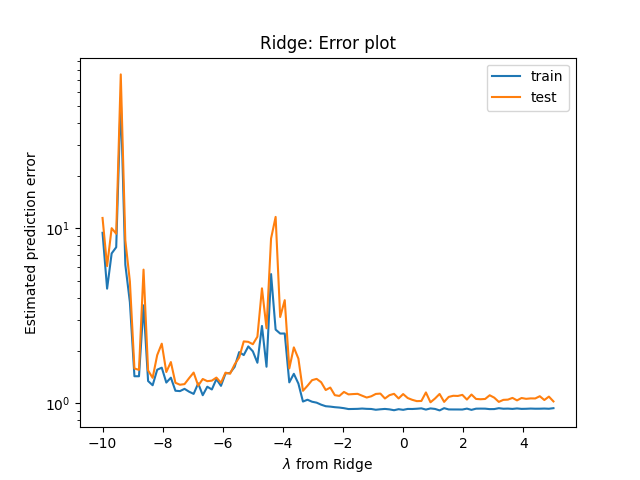
\includegraphics[width=\linewidth, height=7cm]{Figure04.png}
\caption{MSE as a function of lambda for both the test and train data set groups of the Ridge model for the Franke function. We see a local minimum for the negative values of $\lambda$ at around negative seven, but at negative 1 the error reduces to around 1 and stabilises at that value after pasing $\lambda = 0$. This evolution is almist identical for both the train and test datasets.}
\label{MSE_Ridge}
			\end{figure}
We see that both dataset groups MSEs look mostly the same. They fluctuate a little for the negative values with a local minumum at $\lambda = -7$ and reach a minimum around zero where they stabilise. \\
The Bootstrap for the Ridge gives us a plot of the MSE, Bias and Variance as seen in figure \ref{Bootstrap_Ridge}.
			\begin{figure}[H]
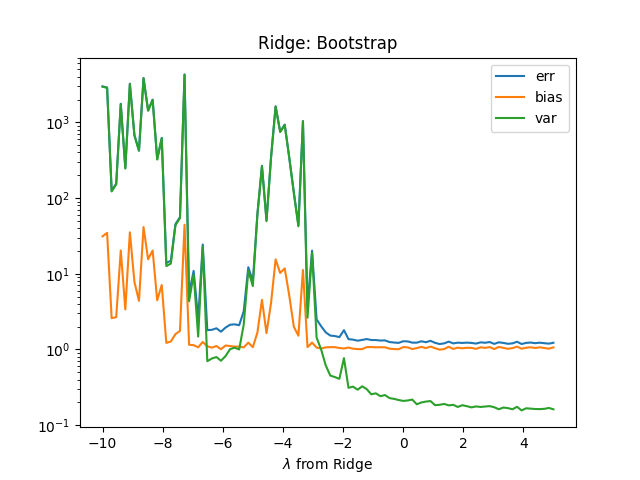
\includegraphics[width=\linewidth, height=7cm]{Figure05.png}
\caption{Bootstrap MSE, bias and variance for Ridge model of the Franke function. The three curves fluctuate erratically until $\lambda = -1$ where they stabilise at a minimum value. the exception is variance which continue to decrease.}
\label{Bootstrap_Ridge}
			\end{figure}
We see all three quantities fluctuate for negative values of lambda, but stabilise after negative 1 for quite a low value except variance which continue to decrease. \\
The CV gives us a MSE which we can compare with the MSE of Bootstrap as we have done for OLS. We have plotted this in figure \ref{CV_Ridge}.
			\begin{figure}[H]
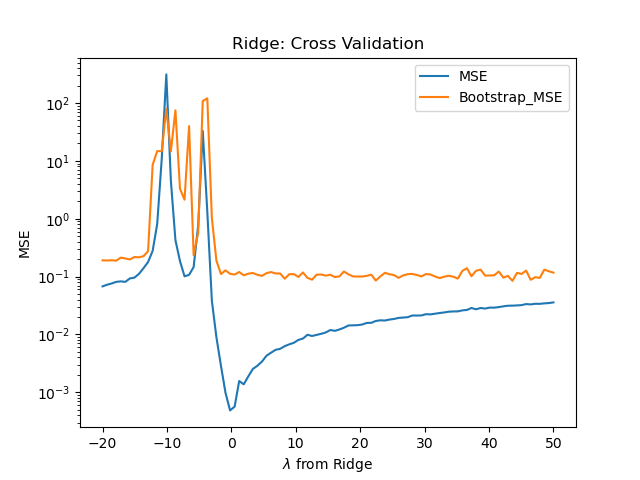
\includegraphics[width=\linewidth, height=7cm]{Figure06.png}
\caption{CV MSE estimate for Ridge compared with the Bootstrap MSE for the Franke function. Both have a local minimum at negative six and stabilise at a minimum after minus one.}
\label{CV_Ridge}
			\end{figure}
We see that this the two curves are almost identical with a local minimum at minus six and a stable minimum after reaching minus one. \\
For the Lasso we get a MSE as a function for the lambda value for both the training and test data. this is plotted in figure \ref{MSE_Lasso}.
			\begin{figure}[H]
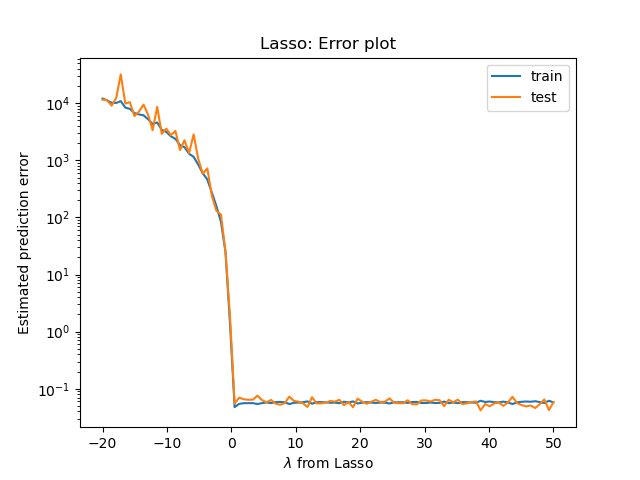
\includegraphics[width=\linewidth, height=7cm]{Figure07.png}
\caption{MSE as a function of lambda for both the test and train dataset groups of the Lasso model with the Franke function. We see a decreasing curve until $\lambda = 0$ where the error stabilises at a minimum.}
\label{MSE_Lasso}
			\end{figure}
We see that both dataset groups have the same evolution, falling down at zero and staying the same after this. \\
The Bootstrap for the Lasso gives us a plot of the MSE, Bias and Variance given in figure \ref{Bootstrap_Lasso}.
			\begin{figure}[H]
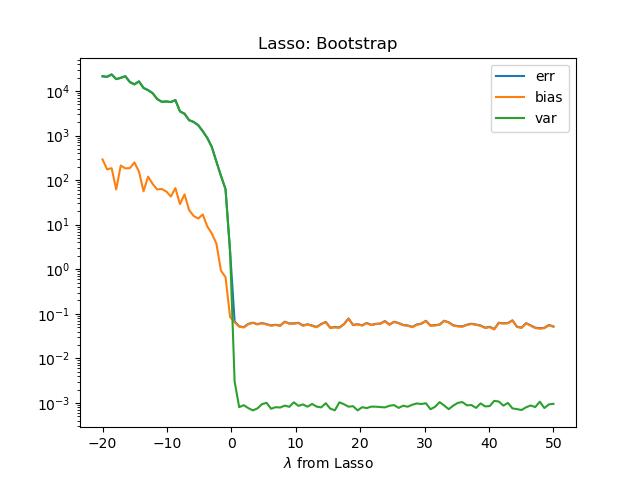
\includegraphics[width=\linewidth, height=7cm]{Figure08.png}
\caption{Bootstrap MSE, bias and variance for Lasso. Has the same general form as the error plot, but we can't see the error because it follows the varians values so much at negative $\lambda$ and bias at positive.}
\label{Bootstrap_Lasso}
			\end{figure}
Varians starts high but drop off a lot at zero. Until then, the error follows this. Then, at lambda equal to zero, the bias passes the variance and the error starts following this. \\
The CV of the Lasso model of the Frake function gives us a MSE which we can compare with the MSE of Bootstrap like earlier, which we see in figure \ref{CV_Lasso}.
			\begin{figure}[H]
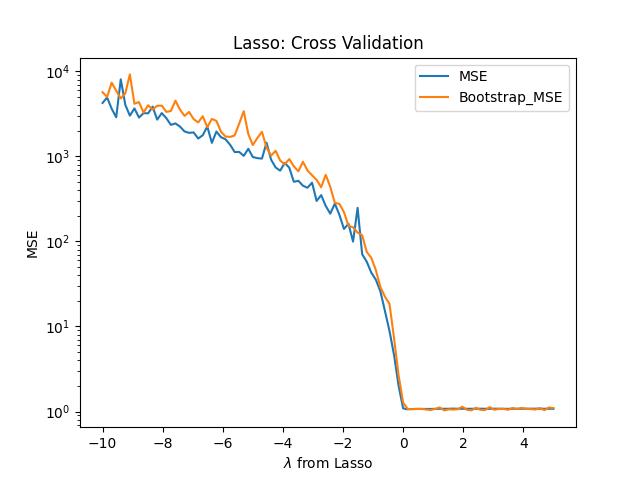
\includegraphics[width=\linewidth, height=7cm]{Figure09.png}
\caption{CV MSE estimate for Lasso compared with the Bootstrap MSE for the Franke function. The CV and Bootstrap look almost identical, falling until zero where they flatten out.}
\label{CV_Lasso}
			\end{figure}
We see that the CV and Bootstrap gives us the same form. They fall of until $\lambda = 0$ where they flatten out. \\
			\subsection{Terrain data}
Then, with the terrain data, we get an OLS, Ridge and Lasso model. For the OLS model we get three analysis plots, using the MSE, Bootstrap and CV methods. We can see these plots in figure \ref{MSE_OLS_terrain}, \ref{Bootstrap_OLS terrain} and \ref{CV_OLS_terrain}.
			\begin{figure}[H]
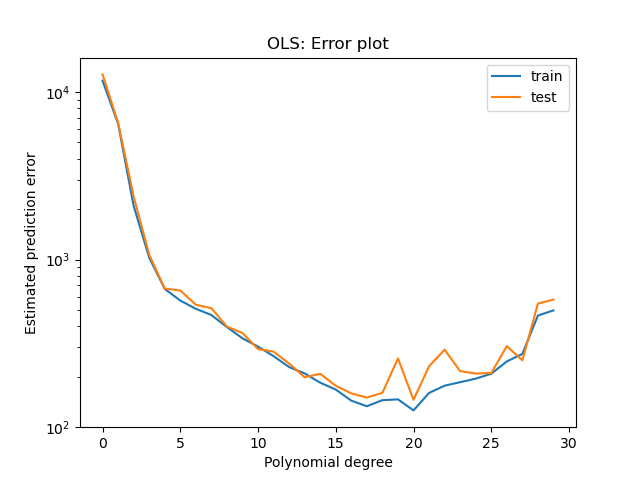
\includegraphics[width=\linewidth, height=7cm]{Figure11.png}
\caption{MSE for OLS for both training and test groups with the terrain dataset. They decrease to a minimum at around 20th degree befor they start to increase again.}
\label{MSE_OLS_terrain}
			\end{figure}
In figure \ref{MSE_OLS_terrain} we see that the terrain data decreases to a minimum around 20th degree befor starting to rise again, for both training and test dataset.
			\begin{figure}[H]
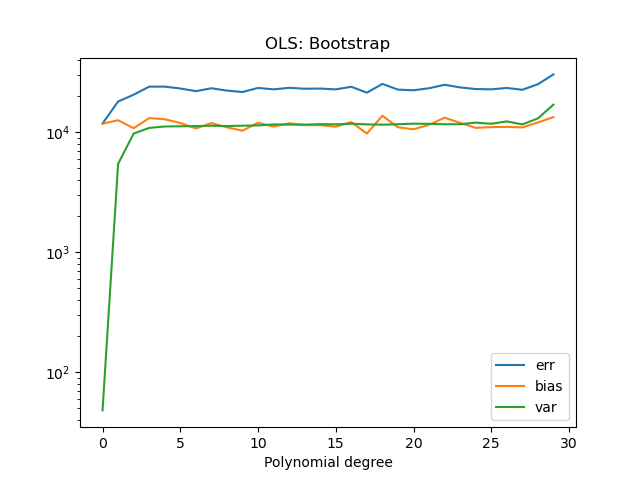
\includegraphics[width=\linewidth, height=7cm]{Figure12.png}
\caption{MSE, Bias and Variance for OLS with the terrain dataset. Bias is just constant with very minor fluctuations for all the polynomial degrees, while error and variance increase in the beginning, flattens out and stays flat until both have a spike at around 25 and then start rising just before 30.}
\label{Bootstrap_OLS terrain}
			\end{figure}
The Bootstrap analysis in \ref{Bootstrap_OLS terrain} show an almost constant flat line for al variable, with an increase in value at the start and a spike at around 25th degree and a rising curve just before 30th.
			\begin{figure}[H]
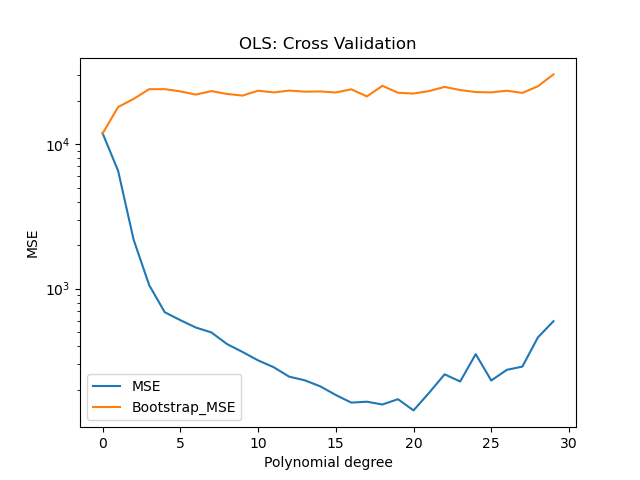
\includegraphics[width=\linewidth, height=7cm]{Figure13.png}
\caption{MSE for OLS for both CV and Bootstrap with the terrain dataset. Here we see a minimum for around 20th degree with a fall off in value before and a rise in value afterwords.}
\label{CV_OLS_terrain}
			\end{figure}
The Cross Validation plot in figure \ref{CV_OLS_terrain} show the same trend as the MSE did, with a minimum at polynomial degree of 20. This is a totally different evolution to the MSE from the Bootstrap. \\
We see that two of the three plots gives us a minimum at around 20th degree. The Bootstrap result is almost constant for all polynomial degrees. \\
For the Ridge analysis of the terrain data, we also get three analysis plots. These are shown in figure \ref{MSE_Lasso_lambda_terrain}, \ref{Bootstrap_Ridge_lambda_terrain} and \ref{CV_Ridge_lambda_terrain}.
			\begin{figure}[H]
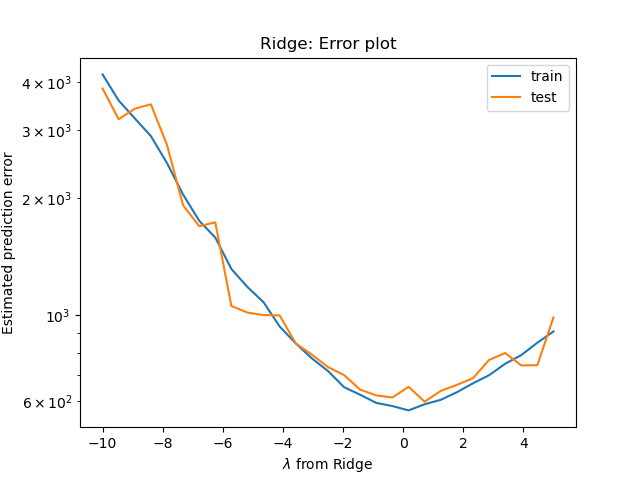
\includegraphics[width=\linewidth, height=7cm]{Figure14.png}
\caption{MSE for Ridge for both training and test groups with the terrain dataset varying with different values of lambda. We see a general decreasing curve until around zero, with a minimum just before at possibly minus a half.}
\label{MSE_Ridge_lambda_terrain}
			\end{figure}
For the MSE plot in figure \ref{MSE_OLS_terrain} we see a trend where both dataset fall and reach a local minimum at around zero with a possible minimum at minus a half, before rising upwards again.
			\begin{figure}[H]
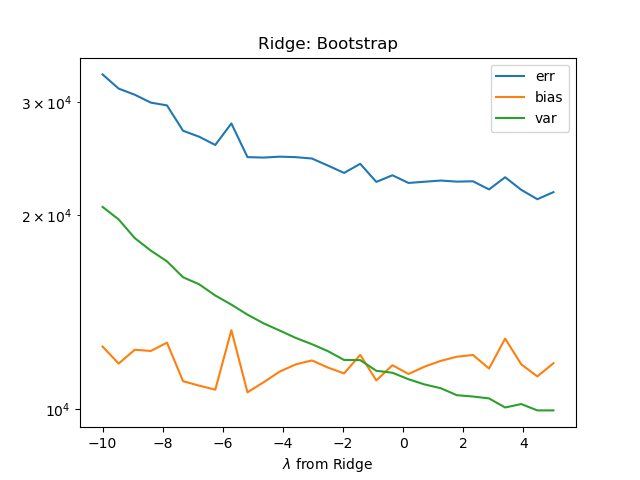
\includegraphics[width=\linewidth, height=7cm]{Figure15.png}
\caption{MSE, Bias and Variance for Ridge with the terrain dataset, for varying lambdas. Here we see that the error and variance decrease slowly for higher values, while the bias just fluctuates around a constant value.}
\label{Bootstrap_Ridge_lambda_terrain}
			\end{figure}
In figure \ref{Bootstrap_Ridge_lambda_terrain} we see the Bootstrap analysis of the Ridge model for different values of lambda. Here the error and the variance drop slowly for higher values of $\lambda$, while the bias fluctuate around the same constant value.
			\begin{figure}[H]
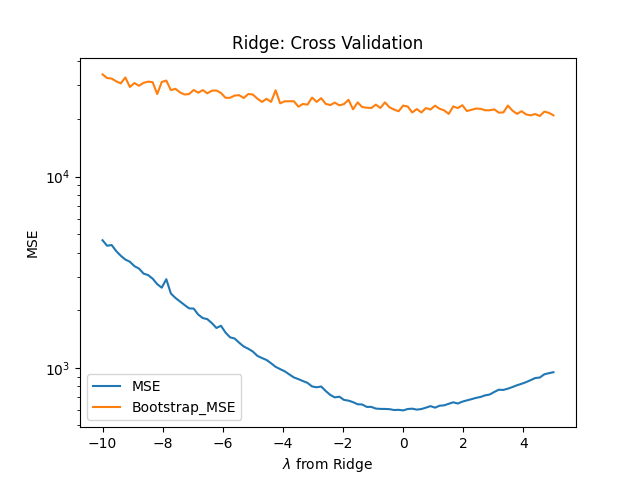
\includegraphics[width=\linewidth, height=7cm]{Figure16.png}
\caption{MSE for Ridge for both CV and Bootstrap with the terrain dataset. Here we see that the CV MSE has a minimum just before zero, while the Bootstrap analysis just falls off for higher values. The general error of the Bootstrap method is also much higher than for the CV.}
\label{CV_Ridge_lambda_terrain}
			\end{figure}
The Cross Validation analysis shown in figure \ref{CV_Ridge_lambda_terrain} decrease and has a minimum just like the MSE had, unlike the Bootstrap error. \\
We see that the MSE and CV gives us a minimum lambda value, but the Bootstraps just drops of for rising values. \\
For the Lasso we get figure \ref{MSE_Lasso_lambda_terrain}, \ref{Bootstrap_Lasso_lambda_terrain} and \ref{CV_Lasso_lambda_terrain}.
			\begin{figure}[H]
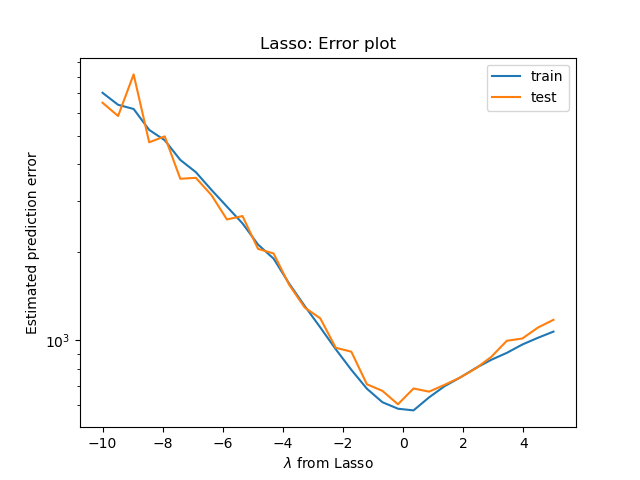
\includegraphics[width=\linewidth, height=7cm]{Figure17.png}
\caption{MSE for Lasso for both training and test groups with the terrain dataset. Here the error decrease sharply until a minimum at about $\lambda = 0.1$ before rising a little slower up again.}
\label{MSE_Lasso_lambda_terrain}
			\end{figure}
In the MSE analysis in figure \ref{MSE_Lasso_lambda_terrain} we see a sharp decrease until a minimum at around $0.1$ when the error start to increase again. The two datasets evolve almost identically.
			\begin{figure}[H]
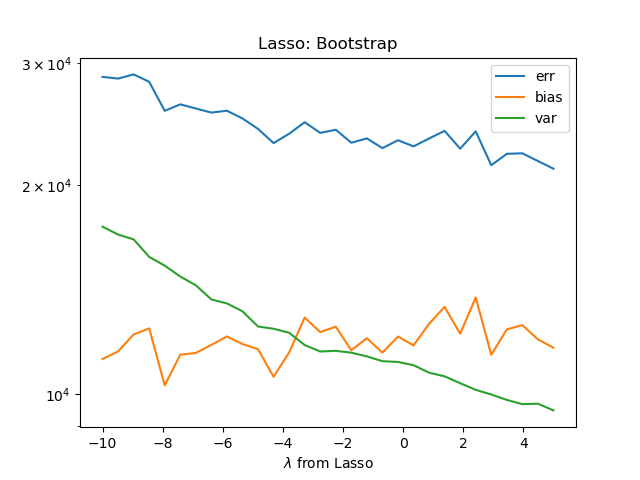
\includegraphics[width=\linewidth, height=7cm]{Figure18.png}
\caption{MSE, Bias and Variance for Lasso with the terrain dataset. The error and variance drop slowly for higher lambda, but the bias varies a around some value. The bias and the error do however seem to increase and decrease at the same lambda values, but with different amounts, giving them a very similar shape.}
\label{Bootstrap_Lasso_lambda_terrain}
			\end{figure}
In the Bootstrap analysis in figure \ref{Bootstrap_Lasso_lambda_terrain} we see the error and variance decrease for higher values of lambda while the bias just varies around a value.
			\begin{figure}[H]
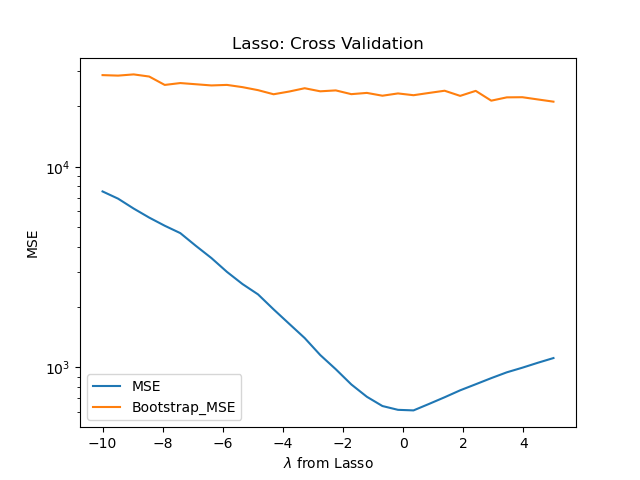
\includegraphics[width=\linewidth, height=7cm]{Figure19.png}
\caption{MSE for Lasso for both CV and Bootstrap with the terrain dataset. The CV MSE drops to a minimum just after zero, unlike the Bootstrap MSE which decreases slowly with no end.}
\label{CV_Lasso_lambda_terrain}
			\end{figure}
Last of all we see that in figure \ref{CV_Lasso_lambda_terrain} we get the same shape as the MSE curves, with a minimum just after zero, unlike the Bootstrap which just decreases. \\
We see that the error and CV gives us a minimum lambda value, but the Bootstraps just drops of for rising values just like we saw for Ridge. \\
Using these optimal values, we get the three analysis plots for Ridge as functions of polynomial degree. These can be seen in figure \ref{MSE_Ridge_poly_terrain}, \ref{Bootstrap_Ridge_poly_terrain} and \ref{CV_Ridge_poly_terrain}.
			\begin{figure}[H]
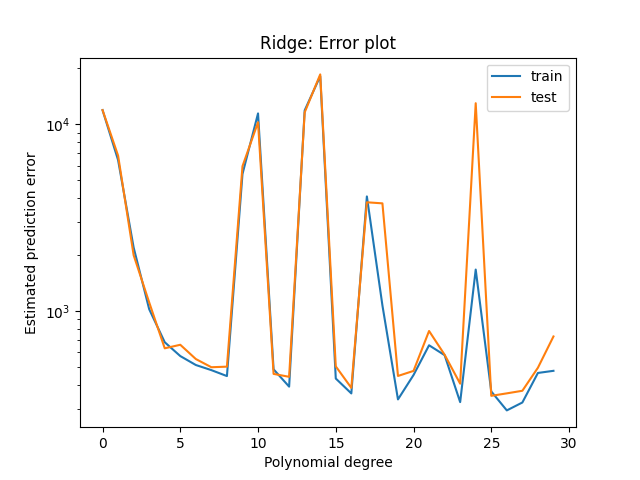
\includegraphics[width=\linewidth, height=7cm]{Figure21.png}
\caption{MSE for Ridge for both training and test groups with the terrain data set as a function of polynomial degree with $\lambda = -0.5$. The MSE decrease sharply until it reaches 8 when it starts to vary up and down, very fast, between maximum and minimum values.}
\label{MSE_Ridge_poly_terrain}
			\end{figure}
			\begin{figure}[H]
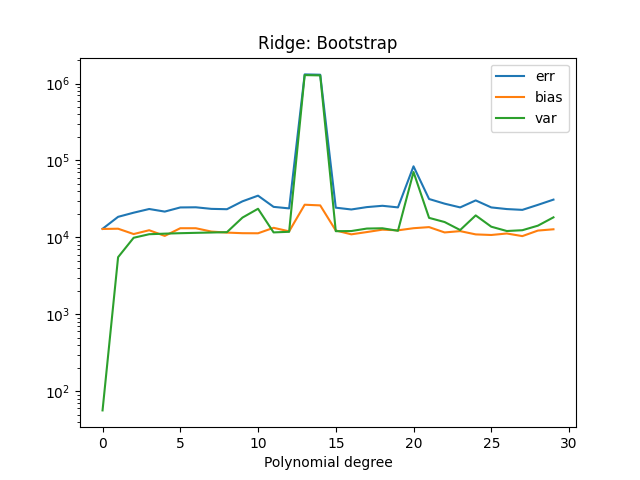
\includegraphics[width=\linewidth, height=7cm]{Figure22.png}
\caption{MSE, Bias and Variance for Ridge with the terrain data set as a function of polynomial degree with $\lambda = -0.5$. Here we see that the error, bias and variance fluctuate a little around a constant value, except for a few spikes in the error and variance where the most notable are at 13th and 20th degree.}
\label{Bootstrap_Ridge_poly_terrain}
			\end{figure}
			\begin{figure}[H]
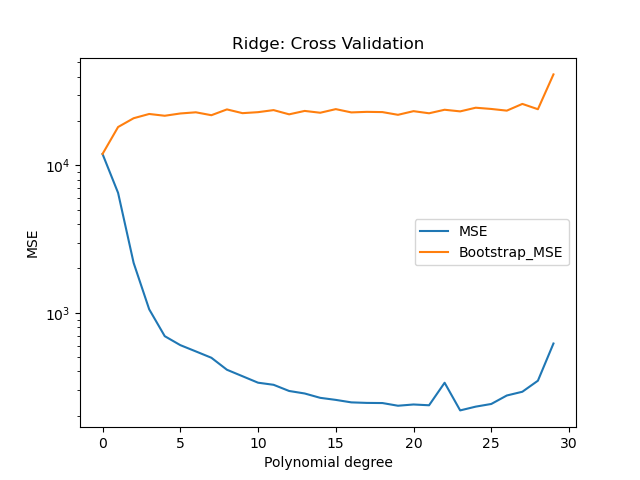
\includegraphics[width=\linewidth, height=7cm]{Figure23.png}
\caption{MSE for Ridge for both CV and Bootstrap with the terrain data set as a function of polynomial degree with $\lambda = -0.5$. The CV MSE has about the same evolution as the MSE, which for one is not that far off from the Bootstrap except for the much larger values.}
\label{CV_Ridge_poly_terrain}
			\end{figure}
We see that the error and CV gives us a local minimum polynomial degree at around 8 before it starts to vary a lot, but the Bootstraps stay constant for most of the plot, with only two large spikes at 13th and 20th degree. \\
For the optimal models we get the following estimated errors \\
			\begin{figure}[H]
				\begin{tabular}{|l|c|c|}
\hline
& OLS & Ridge \\
\hline
MSE & 124.4128106 & 439.1661682 \\
Bootstrap MSE & 22536.47117 & 24029.23005 \\
CV MSE & 155.1733531 & 473.8888207 \\
\hline
				\end{tabular}
\caption{Estimated errors for the two methods, OLS and Ridge with the three different analysis methods. The OLS gives overall better values for all estimates. The Bootstrap values are much higher than the MSE and CV values are.}
\label{Model_Error_Table}
			\end{figure}


		\section{Discussion}
%Were the results what you expected? Are the results significant? - meaning; are the results clear, or are they open to interpretation? How certain can you be of them? What do these results mean in a wider context?
From the analysis of the Franke function we can see that the OLS method doesn't seem to give a best fit value, but it indicates that the best models are all those before 7th polynomial degree. As for the Ridge and Lasso, They both indicate a value very close to zero for the $\lambda$ though they also could be any values above zero as well.The Bootstrap results are odd for every regression method. Though the mean square error looks like it is the sum of the variance and the bias like we would expect, the variance follows the same evolution of the bias, instead of being the opposite like it should. This indicates that there might be a dependence for the variance upon the bias, which there shouldn't be, and that this analysis method here is not as reliable as the other two, It also gives a much higher error than the other two methods, indicating something might be wired, though this might be just a result of it being a different error method. As for the Cross Validation we see about the same evolution as the Error. As for the terrain data, we see almost the same things as for the Franke function, but we can still use the MSE and the CV to find an optimal lambda and polynomial degree. We find $p = 20$ as the optimal for OLS, $\lambda = -0.5$ and $p = 8$ for the Ridge and $\lambda = 0.1$ for the Lasso. However, for the Lasso regression, with the best fit lambda we couldn't get the Lasso regression to converge into a best fit, making this method unavailable. From the calculations of the errors of these best fits, we have that the OLS gives the best fit for our dataset for all the error estimation methods. \\
A problem we have overlooked in this analysis is that we have not calculated confidence interval. This would have been a simple task, just calculating the MSE of the standard deviance if we assumed some distribution model, but we didn't have the time to do so unfortunately. \\
Another problem is that we have chosen to perform the estimation of lambda first, and then the estimation of polynomial degree for the Ridge. This was done to save time, as the calculations where very time consuming. This means we assumes that the two parameters $\lambda$ and $p$ are unrelated, which is not an assumption it is possible to choose without testing, since the $\beta$ variable is a function of $\lambda$ and the higher the polynomial degree, the more betas are in the model.

		\section{Conclusion}
We saw that all the methods estimate a best fit for the Franke function, and for the terrain data, except that the Lasso doesn't converge for the polynomial degree. However we get a best fit for the other two, and from our best fit models we end up with the model best fitting our terrain data is the Ordinary Least Squares model of a $20$th degree polynomial. For future work, it would be useful to find a way to reduce the time consuming part of the code, which seems to be the Lasso and Ridge $\lambda$ analysis such that these can be performed at the same as the polynomial analysis. This would give a more robust model. It would also be useful to look into the Bootstrap method more closely and find out why it behaves so odd compared to the others.
		
\addcontentsline{toc}{section}{Bibliography}
		\begin{thebibliography}{9}
%			\bibitem{<Name of referance>}
%<Name of Author, Name of Author, ...>; \\
%<Title of article> \\
%\url{<URL>} \\
%<Published Date of release> \\
%<Downloaded Date you downloaded webpage>
%			\bibitem{<Name of referance>}
%<Name of Author, Name of Author, ...>; \\
%<Title of article>, <Pages used> \\
%<Year of release>, <Town published>: <Publisher> \\
			\bibitem{USGS}
United States Geological Survey; \\
Earth explorer \\
\url{https://earthexplorer.usgs.gov/} \\
Published 23/09-2014 \\
Downloaded 10/10-2021
			\bibitem{Pinv}
The NumPy community; \\
numpy.linalg.pinv \\
\url{https://numpy.org/doc/stable/reference/generated/numpy.linalg.pinv.html} \\
Published 22/06-2021 \\
Downloaded 10/10-2021
			\bibitem{Lasso}
Pedregosa, F., Varoquaux, G., Gramfort, A., Michel, V., Thirion, B., Grisel, O., Blondel, M., Prettenhofer, P., Weiss, R., Dubourg, V., Vanderplas, J., Passos, A., Cournapeau, D., Brucher, M., Perrot, M., Duchesnay, E.; \\
Scikit-learn: Machine Learning in Python, volum 12, page 2825-2830 \\
Journal of Machine Learning Research, 2011 \\
\url{https://jmlr.csail.mit.edu/papers/v12/pedregosa11a.html}
		\end{thebibliography}
	\end{multicols}
\end{document}